\documentclass[11pt,fleqn]{article}
\usepackage{../cs70,latexsym,epsf, amsmath,amsfonts,graphicx,url}
\lecture{11}
\def\title{Note \the\lecturenumber}

\begin{document}
\maketitle


\section*{Self-Reference and Computability}

In this lecture we will explore the deep connection between proofs and computation. At the heart of this connection is the notion of self-reference, and it has far-reaching consequences to the limit of computations (the Halting Problem) and the foundation of logic in mathematics (G\"odel's incompleteness theorem).



\subsection*{The Liar's Paradox}

Recall that propositions are statements that are either true or false.  We saw before that some statements
are not well defined or too imprecise to be called propositions. But here is a statement that
is problematic for more subtle reasons:
\vspace{-3pt}
$$\text{``All Cretans are liars,"}$$
so said a Cretan in antiquity, thus giving rise to the so-called liar's paradox which has 
amused and confounded people over the centuries. Why? Because if the statement above is true, then the Cretan was lying, which implies the statement is false. But actually the above statement isn't really
a paradox; it simply yields a contradiction if we assume it is true, but if it is false
then there is no problem.

A true formulation of this paradox is the following statement:
\vspace{-3pt}
$$\text{``This statement is false."}$$
Is the statement above true?  If the statement is true, then what 
it asserts must be true; namely that it is false.  But if it is false, then it must be true.  
So it really is a paradox, and we see that it arises because of the self-referential nature of the statement. Around a century ago, this paradox found itself at the center of 
foundational questions about mathematics and computation.

We will now study how this paradox relates to computation.  Before doing so,
let us consider another manifestation of the paradox, created by the great logician
Bertrand Russell. In a village with just one barber, every man keeps himself clean-shaven.
Some of the men shave themselves, while others go to the barber. The barber proclaims:
\vspace{-3pt}
$$\text{``I shave all and only those men who do not shave themselves."}$$
It seems reasonable then to ask the question: Does the barber shave himself? Thinking more carefully about the question though, we see that we are presented with the same self-referential paradox: a logically impossible scenario. If the barber does not shave himself, then according to what he announced, he shaves himself. If the barber
does shave himself, then according to his statement he does not shave himself!



\subsection*{Self-Replicating Programs}

Can we use self-reference to design a program that outputs itself? To illustrate the idea, let us consider how we can do this if we could write the program in English. Consider the following instruction:

\hspace{.3in}\texttt{Print out the following sentence:}

\hspace{.6in}\texttt{``Print out the following sentence:''}

If we execute the instruction above (interpreting it as a program), then we will get the following output:

\hspace{.6in}\textsf{Print out the following sentence:}

Clearly this is not the same as the original instruction above, which consists of two lines. We can try to modify the instruction as follows:

\hspace{.3in}\texttt{Print out the following sentence twice:}

\hspace{.6in}\texttt{``Print out the following sentence twice:''}

Executing this modified instruction yields the output which now consists of two lines:

\hspace{.3in}\textsf{Print out the following sentence twice:}

\hspace{.6in}\textsf{Print out the following sentence twice:}
 
This almost works, except that we are missing the quotes in the second line. We can fix it by modifying the instruction as follows:

\hspace{.3in}\texttt{Print out the following sentence twice, the second time in quotes:}

\hspace{.6in}\texttt{``Print out the following sentence twice, the second time in quotes:''}

Then we see that when we execute this instruction, we get exactly the same output as the instruction itself:

\hspace{.3in}\textsf{Print out the following sentence twice, the second time in quotes:}

\hspace{.6in}\textsf{``Print out the following sentence twice, the second time in quotes:''}



\subsubsection*{Quines and the Recursion Theorem}

In the above section we have seen how to write a self-replicating program in English. But can we do that in a real programming language? In general, a program that prints itself is called a {\em quine},\footnote{Quine is named after the philosopher and logician Willard Van Orman Quine, as popularized in the book {\em ``G\"odel, Escher, Bach: An Eternal Golden Braid''} by Douglas Hofstadter.} and it turns out we can always write quines in any programming language.

As another example, consider the following pseudocode:

\hspace{.3in}\texttt{(Quine ``s'')}

\hspace{.6in}\texttt{(s ``s'')}

The pseudocode above defines a program \texttt{Quine} that takes a string \texttt{s} as input, and outputs\texttt{(s ``s'')}, which means we run the string \texttt{s} (now interpreted as a program) on itself. Now consider executing the program \texttt{Quine} with input \texttt{``Quine''}:

\hspace{.3in}\texttt{(Quine ``Quine'')}

By definition, this will output

\hspace{.6in}\textsf{(Quine ``Quine'')}

which is the same as the instruction that we executed!

This is a simple example, but how do we construct quines in general? The answer is given by the {\em recursion theorem}. The recursion theorem states that given any program $P(x,y)$, we can always convert it to another program $Q(x)$ such that $Q(x) = P(x,Q)$, i.e., $Q$ behaves exactly as $P$ would if its second input is the description of the program $Q$. In this sense we can think of $Q$ as the ``self-aware'' version of $P$, since $Q$ essentially has access to its own description.




\subsection*{The Halting Problem}

Are there tasks that a computer cannot perform?  For example, we would like to ask the 
following basic question 
when compiling a program: does it go into an infinite loop? In 1936, Alan Turing showed
that there is no program that can perform this test.  The proof of this remarkable fact 
is very elegant and combines two ingredients: self-reference (as in the liar's paradox), 
and the fact that we cannot separate
programs from data. In computers, a program is represented by a string of bits just as
integers, characters, and other data are.  The only difference is in how the string of 
bits is interpreted.

We will now examine the Halting Problem. Given the description of a program and its input, 
we would like to know if the program ever halts when it is executed on the given input.  
In other words, we would like to write a program \texttt{TestHalt} that behaves as follows:
$$
\texttt{TestHalt(P,x)} = \left\{ 
\begin{array}{cc}
$``yes"$,&\mbox{ if }$ program $P$ halts on input $x\\
$``no"$, &\mbox{ if }$ program $P$ loops on input $x
\end{array}\right.
$$

\noindent Why can't such a program exist?  First, let us use the fact that a program
is just a bit string, so it can be input as data.  This means that it is perfectly
valid to consider the behavior of \texttt{TestHalt(P,P)}, which
will output ``yes" if $P$ halts on $P$, and ``no" if $P$ loops forever on~$P$.
We now prove that such a program cannot exist.
\vspace{.1cm}

\textbf{Proof:} Define the program

\hspace{.5in} \texttt{Turing(P)}

\hspace{.7in} \texttt{if TestHalt(P,P) = ``yes'' then loop forever}

\hspace{.7in} \texttt{else halt}
\vspace{.1cm}

\noindent So if the program $P$ when given $P$ as input halts, then \texttt{Turing(P)} loops forever;
otherwise, \texttt{Turing(P)} halts.  Assuming we have the program \texttt{TestHalt}, we can easily use
it as a subroutine in the above program \texttt{Turing}.

Now let us look at the behavior of \texttt{Turing(Turing)}. There are two cases: either it halts, 
or it does not.  If \texttt{Turing(Turing)} halts, then it must be the case that 
\texttt{TestHalt(Turing,Turing)} returned ``no."
But by definition of \texttt{TestHalt}, that would mean that \texttt{Turing(Turing)} should not have halted. In the second case, if
\texttt{Turing(Turing)} does not halt, then it must be the case that \texttt{TestHalt(Turing, Turing)}
returned "yes," which would mean that \texttt{Turing(Turing)} should have halted. 
In both cases, we arrive at a contradiction
which must mean that our initial assumption, namely that the program \texttt{TestHalt} exists, 
was wrong.  Thus, \texttt{TestHalt} cannot exist, so it is impossible for a program to check 
if any general program halts.
\qed

\vspace{.1in}

What proof technique did we use? This was actually a proof by diagonalization, the same technique that we used in the previous lecture to show that the real numbers are uncountable. Why? Since 
the set of all computer programs is countable (they are, after all, just finite-length
strings over some alphabet, and the set of all finite-length strings is countable), we can
enumerate all programs as follows (where $P_i$ represents the $i^{\rm th}$ program):

%\vspace{.4in}

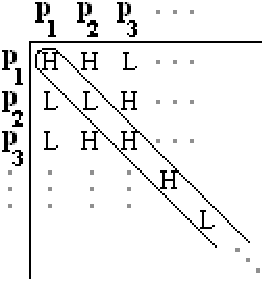
\includegraphics[bb = -40 0 0 100, scale=0.7]{halt3}

The $(i,j)^{\rm th}$ entry in the table above is~H if program $P_i$ halts on input~$P_j$, and~L if it does not halt.
Now if the program \texttt{Turing} exists it must occur somewhere on our list of programs, say as $P_n$.
But this cannot be, since if the $n^{\rm th}$ entry in the diagonal is~H, meaning that $P_n$
halts on~$P_n$, then by its definition \texttt{Turing} loops on~$P_n$; and if 
the entry is~L, then by definition \texttt{Turing} halts on~$P_n$.  Thus the behavior of \texttt{Turing} 
is different from that of~$P_n$, and hence \texttt{Turing} does not appear on our list.
Since the list contains all possible programs, we must conclude that the program
\texttt{Turing} does not exist.  And since \texttt{Turing} is constructed by a simple modification of
\texttt{TestHalt}, we can conclude that \texttt{TestHalt} does not exist either.  Hence the Halting
Problem cannot be solved.

In fact, there are many more cases of questions we would like to answer about a program, 
but cannot. For example, we cannot
know if a program ever outputs anything or if it ever executes a specific line. We also cannot check if two programs produce the same output. We cannot even
check to see if the program is a virus.  These issues are explored in greater detail in
the advanced course CS172 (Computability and Complexity).


\subsubsection*{The Easy Halting Problem}

As noted above, the key idea in establishing the uncomputability of the Halting Problem is self-reference: Given a program $P$, we want to check whether $P(P)$ halts. But in practice, how often do we want to execute a program with its own description as input? Is it possible that if we disallow this kind of self-reference, we can answer the Halting Problem?

That is, given a program $P$, what if we ask: ``Does $P$ halts on input $0$?'' This looks easier than the Halting Problem (hence the name Easy Halting Problem), since we only need to check whether $P$ halts on a specific input $0$, instead of an arbitrary given input. However, it turns out this easier problem is still uncomputable. We prove this claim by showing that if we can solve the Easy Halting Problem, then we can also solve the Halting Problem; since we know the Halting Problem is uncomputable, this implies the Easy Halting Problem must also be uncomputable.

Specifically, suppose we have a program \texttt{TestEasyHalt} that answers the Easy Halting Problem:
$$
\texttt{TestEasyHalt(P)} = \left\{ 
\begin{array}{cc}
$``yes"$,&\mbox{ if }$ program $P$ halts on input $0\\
$``no"$, &\mbox{ if }$ program $P$ loops on input $0
\end{array}\right.
$$
Then we can use \texttt{TestEasyHalt} as a subroutine in the following algorithm that solves the Halting Problem:

\hspace{.5in} \texttt{Halt(P,x)}

\hspace{.7in} \texttt{define a program P' that returns P(x) on input 0}

\hspace{.7in} \texttt{return TestEasyHalt(P')}
\vspace{.1cm}

The algorithm \texttt{Halt} constructs another program $P'$, which depends on both the original program $P$ and the original input $x$, such that when we call $P'(0)$ we return $P(x)$. An example of such a program $P'$ can simply be:

\hspace{.5in} \texttt{P'(y)}

\hspace{.7in} \texttt{return P(x)}
\vspace{.1cm}

That is, the new program $P'$ ignores the input $y$ and always returns $P(x)$. Then we see that $P'(0)$ halts if and only if $P(x)$ halts. Therefore, if we have such a program \texttt{TestEasyHalt}, then \texttt{Halt} will correctly answer the Halting Problem. Since we know there cannot be such a program \texttt{Halt}, we conclude \texttt{TestEasyHalt} does not exist either.

The technique that we use here is called a {\em reduction}. Here we are reducing one problem ``Does $P$ halt on $x$?'' into another problem ``Does $P'$ halt on $0$?'', in the sense that if we know how to answer the second problem, then we can use that knowledge to construct an answer for the first problem. This implies that the second problem is actually as difficult as the first, despite the apparently simpler description of the second problem.



\subsection*{G{o}del's Incompleteness Theorem}

In 1900, the great mathematician David Hilbert posed the following two questions about the foundation of logic in mathematics:
\begin{enumerate}
\vspace{-6pt}
  \item Is arithmetic consistent?
\vspace{-3pt}
  \item Is arithmetic complete?
\end{enumerate}

To understand the questions above, we recall that mathematics is a formal system based on a list of axioms (for example, Peano's axioms of the natural numbers, axiom of choice, etc.) together with rules of inference. The axioms provide the initial list of true statements in our system, and we can apply the rules of inference to prove other true statements, which we can again use to prove other statements, and so on.

The first question above asks whether it is possible to prove both a proposition $P$ and its negation $\neg P$. If this is the case, then we say that arithmetic is {\em inconsistent}; otherwise, we say arithmetic is {\em consistent}. If arithmetic is inconsistent, meaning there are false statements that can be proved, then the entire arithmetic system will collapse because from a false statement we can deduce anything, so every statement in our system will be vacuously true.

The second question above asks whether every true statement in arithmetic can be proved. If this is the case, then we say that arithmetic is {\em complete}. We note that given a statement, which is either true or false, it can be very difficult to prove which one it is. As a real-world example, consider the following statement, which is known as Fermat's Last Theorem:
$$\forall \, n \ge 3, ~ \not\exists \: x,y,z \in \mathbb{Z}, \:~ x^n + y^n = z^n.$$
This theorem was first stated by Pierre de Fermat in 1637,\footnote{Along with the famous note: ``I have discovered a truly marvelous proof of this, which this margin is too narrow to contain.''} but it has eluded proofs for centuries until it was finally proved by Andrew Wiles in 1994.

In 1928, Hilbert formally posed the questions above as the Entscheidungsproblem. Most people believed that the answer would be ``yes,'' since ideally arithmetic should be both consistent and complete. However, in 1930 Kurt G\"odel proved that the answer is in fact ``no'': Any formal system that is sufficiently rich to formalize computation is either inconsistent (there are false statements that can be proved) or incomplete (there are true statements that cannot be proved). G\"odel proved his result by exploiting the deep connection between proofs and computation, but it was not until 1936 that Turing formalized the definition of computation via the notion of Turing machines and computability.

In the rest of this note, we will first understand the essence of G\"odel's proof, and then we will provide an easier proof using the Halting Problem.


\subsubsection*{Sketch of G\"odel's Proof}

Suppose we have a formal system $F$, which consists of a list of axioms and rules of inference, and assume $F$ is sufficiently expressive that we can use it to express computation. Arithmetic is an example of such a system $F$.

Now suppose we can write a sentence:
$$S(F) = \text{``This sentence is not provable in $F$.''}$$
Once we have this sentence, there are two possibilities:
\begin{enumerate}
  \item Case 1: $S(F)$ is provable. Then the sentence $S(F)$ is true, but by inspecting the content of the sentence itself, we see that this implies $S(F)$ should not be provable. Thus, $F$ is inconsistent in this case.
  \item Case 2: $S(F)$ is not provable. By construction, this means the sentence $S(F)$ is true. Thus, $F$ is incomplete in this case, since there is a true statement (namely, $S(F)$) that is not provable.
\end{enumerate}

To complete the proof, it now suffices to construct such a sentence $S(F)$. This is the difficult part of G\"odel's proof, which requires a clever encoding (G\"odel numbering) of symbols and propositions as natural numbers.



\subsubsection*{Proof via the Halting Problem}

Let us now see how we can prove G\"odel's result by reduction to the Halting Problem. Here we proceed by contradiction: Suppose arithmetic is both consistent and complete; we will use this assumption to solve the Easy Halting Problem, which we have seen is as difficult as the Halting Problem.

Recall that in the Easy Halting Problem we want to decide whether a given program $P$ halts on input $0$. Let $S$ denote the sentence ``$P$ halts on input $0$.'' This is a sentence in arithmetic, and because we assume arithmetic is consistent and complete, we know that $S$ is either true or false, and there is a proof either way.

Recall also that a proof is simply a finite binary string. How many proofs are there? There are countably many, so we can enumerate them and go through them one by one. Now define the program $M$ as follows:

\hspace{.5in} \texttt{M(P)}

\hspace{.7in} \texttt{for every proof x:}

\hspace{.9in} \texttt{if x is a proof that P halts on 0, then output ``yes''}

\hspace{.9in} \texttt{if x is a proof that P does not halt on 0, then output ``no''}

\vspace{.1cm}

The program $M$ takes as input the program $P$, and proceed to check every possible proof until it finds one that proves either $P(0)$ halts, or $P(0)$ does not halt. By assumption, we know there is always such a proof, so the algorithm $M$ will terminate in finite time, and it will correctly answer the Easy Halting Problem. Since we have established that there cannot be such a program $M$, our initial assumption must be wrong, so it is not true that arithmetic is both consistent and complete.

Note that here we rely on the fact that given a proof, we can have a program that mechanistically check whether it is a valid proof for our proposition, and the argument above shows how we can use this to answer questions about the limit of computability. This is a manifestation of the intimate ties between proofs and computation in a deep level.











\end{document}
